\documentclass[11pt,a4paper]{article}

\usepackage[T1]{fontenc}
\usepackage[utf8]{inputenc}
\usepackage[a4paper,top=2.0cm,bottom=2.2cm,left=2.4cm,right=2.4cm]{geometry}
\usepackage{amsmath}
\usepackage{booktabs,tabularx,array}
\usepackage{xcolor}
\usepackage{graphicx}
\usepackage{float}
\usepackage{caption}
\usepackage{enumitem}
\usepackage{titlesec}
\usepackage{xurl}
\usepackage{hyperref}
% File paths set in \texttt are single unbreakable boxes, and a long one
% (sweep/appworld_rate_limit_cost.json) can overrun the margin no matter how the
% surrounding prose is worded. \code sets them in typewriter but lets the line
% break inside, at no hyphen -- a hyphen would read as part of the path.
\DeclareUrlCommand\code{\urlstyle{tt}}
\usepackage{tikz}
\usetikzlibrary{arrows.meta,positioning,fit,backgrounds,calc}
\usepackage{microtype}

% Three roles only: ink for text, one accent, one rule gray.
% Diagram groups are separated by outline, fill tint and line style
% rather than by hue, so the figures survive black-and-white printing.
\definecolor{ink}{HTML}{1A1D23}
\definecolor{accent}{HTML}{1F3A5F}
\definecolor{muted}{HTML}{6B7280}
\definecolor{rulegray}{HTML}{C3C8D0}

\hypersetup{
  colorlinks=true,
  linkcolor=ink,
  citecolor=accent,
  urlcolor=accent,
  pdfauthor={Jinao Wang},
  pdftitle={Verifiable Multi-Agent RL Task Construction from Information Seams and Permission Partitions}
}

\setlength{\parskip}{0pt}
% Long \texttt paths (sweep/appworld_protocol.json) are single unbreakable boxes,
% and English has none of the CJK version's break-anywhere slack. Give TeX real
% stretch on the final pass so those paragraphs fit, rather than letting them run
% into the margin -- build_report.sh treats an overfull box as unshippable.
\setlength{\emergencystretch}{1.5em}
\renewcommand{\arraystretch}{1.25}
\captionsetup{font=small,labelfont=bf}
\setcounter{secnumdepth}{2}
\setcounter{tocdepth}{2}

\titleformat{\section}{\large\bfseries\color{ink}}{\thesection}{0.7em}{}
\titleformat{\subsection}{\normalsize\bfseries\color{ink}}{\thesubsection}{0.7em}{}
\titlespacing*{\section}{0pt}{1.5em}{0.6em}
\titlespacing*{\subsection}{0pt}{1.0em}{0.4em}
\pagestyle{plain}

\begin{document}

\hypersetup{pageanchor=false}
\thispagestyle{empty}

\vspace*{1.5cm}
% Hyphenation off and ragged right: at 21pt the second line broke as
% "Permission Par-titions", and a hyphen in a title reads as a typo rather than
% as typesetting. The line breaks here are chosen, not discovered.
\noindent{\bfseries\fontsize{19}{25}\selectfont\color{ink}
\hyphenpenalty=10000\exhyphenpenalty=10000\raggedright
Verifiable Multi-Agent RL Task Construction\\[0.15em]
from Information Seams and Permission Partitions\par}

\vspace{0.55cm}
\noindent{\large\color{ink}A method for turning an agentic task database into multi-agent RL tasks, instantiated on AppWorld\par}

\vspace{0.9cm}
\noindent{\large\color{ink}Jinao Wang\par}
\vspace{0.35em}
\noindent{\color{muted}Multi-Agent Task Forge\par}
\vspace{0.2em}
\noindent{\color{muted}17 July 2026\par}

\vspace{0.5cm}
\noindent{\color{rulegray}\rule{0.32\textwidth}{0.4pt}}

\vspace{0.45cm}
\noindent\begin{minipage}{0.9\textwidth}
\setlength{\parindent}{0pt}
{\bfseries Abstract}\hspace{0.6em}This report presents a method, and one substrate carried through it end to end. The method takes an agentic task database that was never meant for multi-agent work and turns its single-agent tasks into training tasks that cannot be finished without collaboration --- without writing a new task, a new environment, or a new verifier. It asks four things of a database and nothing else: a verifier somebody else wrote, an installable world, a reference solution per task, and an action surface that divides along role boundaries. Any database clearing those admits the method; AppWorld is the one this report runs, and \S\ref{sec:substrate} states plainly that it is the only one. Concretely, on AppWorld: read the 147 tasks that carry ground truth, parse their reference solutions, and keep, via one forward taint pass, the 39 whose facts genuinely cross an app boundary. The roster comes from the apps the reference solution actually touched, rather than from padding a task out to look multi-agent. Each task is then wrapped in a permission partition: the Main agent holds no app API at all and can only delegate, while the verifier and the ground truth stay on a side it cannot reach. Whether the task is done is still decided by AppWorld's own database-state checks, and the reward is the fraction of state requirements that pass. No LLM judge is involved.

\vspace{0.5em}
The cost structure of this method is lopsided, and that is what determines how it scales. Selecting tasks, deriving rosters, and rendering task directories are all static analysis with no model calls: spreading 39 tasks into 78 Harbor task directories is one command and a few minutes. The bills come afterwards. A task can only ship if a reference solution proves it solvable, and those are currently written by hand; a cell only counts once enough seeds have been run to show whether it produces a non-degenerate training signal. So the way up is not to keep adding knobs. It is to automate reference-solution generation first (\S\ref{sec:refcost} --- the seam analysis has already computed its skeleton), then to widen the source pool: the ceiling on this dimension is 13 independent task families, not 39 tasks, and certainly not 78 directories.
\end{minipage}

\clearpage
\thispagestyle{empty}
{\setlength{\parskip}{0pt}
\renewcommand{\contentsname}{\normalsize\bfseries Contents}
\tableofcontents}

\clearpage
\hypersetup{pageanchor=true}
\pagenumbering{arabic}

\section{Problem and Goal}

A task usable for reinforcement learning needs at least three parts: the instruction the model receives, the environment it can interact with, and the reward issued once the episode ends. Single-agent tasks are usually easy to verify --- check whether a file was created, whether a database row changed, whether the tests pass. Multi-agent tasks are harder, because we care about more than the end result: we want the model to hand subtasks to the right role and to move the necessary facts between roles.

There is an easy mistake here. Add a few roles and a group chat, and the task looks multi-agent. But if the Main agent still holds every tool, or if any sub-agent could finish the task alone, then the roles are set dressing and produce no new learning signal. Score the transcript on whether it \emph{looks} collaborative instead, and the reward becomes subjective and impossible to scale.

So this project narrows the goal: start from real tasks that already have a trustworthy verifier, then use permission and information constraints to make collaboration \emph{necessary} for finishing. The model must demonstrate coordination, but the reward is still decided solely by the end state.

Stated at the level it is meant to be reused at, that goal is a \textbf{method} rather than a dataset. No corpus of multi-agent traces with environments and free verifiers exists, so anyone building this data must manufacture the multi-agent structure themselves; the only real decision is \emph{which layer} they manufacture. Manufacture the verifier and the mistakes become invisible, because your own tests will agree with your own errors --- \S\ref{sec:invariant} is that failure, measured. Manufacture only \emph{constraints}, which change who may do what and never what counts as done, and the failure mode becomes a task that is too easy or too hard: visible, and priceable by the criterion of \S\ref{sec:criterion}. The rest of this report is that method in four moves --- admit a database (\S\ref{sec:substrate}), mine its seams (\S\ref{sec:select}), constrain access (\S\ref{sec:wrap}), accept only the cells that land between the floor and the control (\S\ref{sec:criterion}) --- and one database, AppWorld, carried through all four.

\section{Capability Selection and Learning Order}

Multi-agent systems involve many capabilities. To keep the training signal legible, this design first picks the ones that can be verified from environment outcomes and that compose in layers. MAST groups common failures into system design, inter-agent misalignment, task verification and termination, and related classes~\cite{cemri2025mast}; MultiAgentBench shows that star, chain, tree and graph topologies impose different coordination demands~\cite{zhu2025multiagentbench}. At the data-construction stage, though, changing every factor at once is the wrong move.

\begin{table}[H]
\centering
\small
\caption{Capabilities currently prioritised for training}
\label{tab:capabilities}
\begin{tabularx}{\textwidth}{>{\raggedright\arraybackslash}p{2.9cm} X >{\raggedright\arraybackslash}p{4.3cm}}
\toprule
Capability & What the model must learn & How failure shows up\\
\midrule
Decomposition and dependency recognition & Break a goal into executable subtasks and work out which intermediate results must come first & A necessary app is skipped, the order is wrong, a downstream step lacks its upstream fact\\
Role assignment & Route each subtask to the role whose information and tools fit it & The request goes to the wrong role, or a role is asked to read what it cannot see\\
Cross-role communication & Carry entities, date ranges and prior results into the delegation, so local execution serves the global goal & The sub-agent satisfies its own request, but the final world state is still wrong\\
Parallel scheduling & Cut needless serial waiting while respecting dependencies and resource limits & Resource conflicts, dropped tasks, unmet dependencies, or an inflated makespan\\
\bottomrule
\end{tabularx}
\end{table}

The first three capabilities in Table~\ref{tab:capabilities} are exercised directly by the current delivery. Parallel scheduling is the exception. It is listed because it belongs to the same family --- verifiable from environment state --- but this AppWorld-based delivery does not cover it: the sidecar is single-threaded (AppWorld's world is not thread-safe), delegation calls block serially, and the terminal scalar $r=N_{\mathrm{pass}}/N$ has no way to price makespan. Training it needs a runtime that can express concurrency, which is out of scope here --- the same reason Theory of Mind is not listed as its own dimension below.

These capabilities suit layered training. The first layer asks only that the model identify the roles and delegate once, correctly. The second adds a cross-app dependency, so the Main must carry an upstream result downstream. The third hides the roles' capability documentation, forcing the model to work out who might know what. Only later come delegation budgets, more roles, and richer topologies. One clarification is due here: the third layer already implies Theory of Mind --- judging \emph{who might know what} is exactly modelling another role's knowledge state, and the failure criterion for ``cross-role communication'' in Table~\ref{tab:capabilities} is the same thing seen from the other side, where the Main assumes the sub-agent knows as much as it does and issues a delegation the sub-agent cannot act on. The reason Theory of Mind and dynamic recovery are still not separate dimensions is not that they are unimportant. It is that the current reward is a single terminal scalar and cannot attribute one failure to that link alone.

That limitation belongs to this design, not to the capability. By the rule of \S\ref{sec:invariant} --- the sin is the unmeasured verifier, not the language model --- attribution is not hopeless: a teacher model that reads the ledger and decides whether a failure lay in decomposition, routing or communication is entirely buildable. It is a self-designed judge, so it needs a validation study (agreement against human labels), not a prohibition. What is unacceptable is using one \emph{without measuring it}, which is precisely what v1 did with that one line of division. So the route is: the terminal scalar stays the only training reward, and the teacher model is used for \emph{diagnosis} and curriculum design; once its attribution accuracy has been measured, we can discuss whether it may enter the reward. This report has not done that step, so the table above lists only terminally verifiable capabilities.

\begin{quote}
\small
\noindent The suggested progression is: single-shot role routing $\rightarrow$ star + visible capability docs $\rightarrow$
star + role names only $\rightarrow$ limited budget and multi-level dependencies $\rightarrow$ chain/tree and runtime faults.
\end{quote}

The current implementation and experiments reach the third layer. The last two have a clear construction path, but each must be shown solvable and shown to add difficulty before it enters a training set.

\section{From Single-Agent Task to Collaborative Task}
\label{sec:wrap}

The method fits in one sentence: \emph{keep the task and the verifier; restructure only how agents reach the task.}

The original task already has a user instruction, an interactive environment, and a programmatic verifier. Forging adds coordination constraints --- communication topology, role visibility, delegation budget --- in a layer outside it. However the model decomposes and communicates, the original environment tests still decide whether the task is done.

More precisely, write the original task as
\[
  \tau=(x,\mathcal{E},J),
  \qquad
  \mathcal{E}_c=W(\mathcal{E};c),
  \qquad
  \tau_c=(x,\mathcal{E}_c,J).
\]
Here $x$ is the user instruction, $\mathcal{E}$ the environment, $J$ the programmatic verifier. $W$ is a wrapping operator that acts \emph{only on the environment}: it does not rewrite the instruction and does not rewrite the verifier --- $x$ and $J$ are literally identical on both sides. That is the entire source of this method's safety, and the only thing separating it from ``design your own verifier''. The constraint
\[
  c=(P,V,G,B)
\]
has four components: $P$, the permission partition (which role holds which app's API); $V$, role visibility (what the Main may know about the roles); $G$, the communication graph (who may message whom); and $B$, the delegation budget.

Three notes. First, $P$ refers to the \emph{structure} of the partition --- the Main holds no API, each specialist binds to exactly one app. Which apps those are is not a knob; it is determined by the reference solution (\S\ref{sec:select}). Second, $P$ is the most fundamental of the four: without it the Main can bypass coordination and simply do the task, and the other three become moot. Third, $J$ is unchanged word for word, but what it reads is the terminal state inside the sidecar; $W$ simultaneously guarantees that neither $J$ nor the ground truth exists anywhere on the agent's filesystem (\S\ref{sec:boundary}).

This is close in spirit to SWE-smith's principle of extending software tasks with the tests that already exist~\cite{yang2025swesmith}: reuse verification logic that is already trustworthy rather than designing fresh judging logic per task. The whole forging process reduces to three steps: identify cross-app dependencies in real tasks, derive the roster from those dependencies, and wrap the same task into different coordination configurations.

\subsection{Selecting tasks from real dependencies}
\label{sec:select}

AppWorld provides 9 everyday apps, 457 APIs and 750 complex tasks (the currently published dataset actually contains 732), and uses database-state tests to decide both whether a task was completed and whether it caused unintended modifications~\cite{trivedi2024appworld}. This repository reads the 147 tasks in train and dev that carry full ground truth and analyses which apps their reference solutions actually call.

The roster is decided entirely by the task itself. If a task's reference solution calls both phone and venmo, it naturally corresponds to two specialists. \texttt{supervisor.complete\_task}, used to submit the answer, does not count as a role, because it supplies no business information. Under that rule, 51 of the 147 tasks genuinely need at least two apps; the rest are discarded outright rather than padded with an irrelevant role to manufacture a multi-agent shape.

\subsection{Turning a single-agent task into a collaborative one}

The wrapped environment holds one Main agent and several app-bound sub-agents. The Main sees the user goal but holds no app API; the phone specialist can reach only phone, the venmo specialist only venmo. Sub-agents know only the local request the Main sent them, never the whole task.

Take one task from the current delivery: ``On my Venmo social feed, like all of today's transactions involving my roommates.'' The Main must first ask phone which contacts are roommates, then hand that list of names, together with the date range, to venmo. Neither sub-agent can finish the task alone: phone knows the relationships but cannot like anything; venmo can like transactions but does not know who the roommates are. The task therefore carries a clean dependency chain of its own:
\[
  \text{phone yields roommate names}
  \longrightarrow
  \text{Main carries names and range}
  \longrightarrow
  \text{venmo iterates and acts}.
\]

This construction tests the model along three axes at once: discovering which role holds which information, ordering the subtasks correctly, and carrying the context the downstream role actually needs. But the terminal reward can only judge whether the whole thing got done; it cannot attribute one failure to one of those axes (see \S\ref{sec:verifyfirst}). The prompt remains a natural-language task, and the dependency graph exists only in the environment and the reference solution --- it is never shown to the model.

\section{The Forging Method: Four Elements}

SWE-smith's leverage is not clever bug injection. It is that it never designs a verifier: break a repository that used to work, and let the repository's own tests decide whether the fix is right~\cite{yang2025swesmith}. Taken apart, the method has only four elements: an invariant (the repo's tests), a set of operators (five ways to produce candidates), a criterion (the patch counts only if tests that used to pass go red), and a measured yield for each operator (56\%, 35\%, 40.2\%, 33.8\%, 96.9\%).

Any forging method must answer the same four questions. This section places the present design against those four elements and names the gaps.

\subsection{Invariant: inherit the verifier; if you must build one, measure it first}
\label{sec:invariant}

Forging can act at two levels: design the world and the verifier, or design only the constraints. The failure modes are not symmetric. Choose the wrong constraint and the task is too easy or too hard --- which is measurable. Design the verifier wrong and the reward measures the wrong thing --- which is invisible, because your own tests will agree with your own mistake. This design therefore touches only the latter: constraints change \emph{who may do what} and never touch \emph{what counts as done}. That is not laziness; it trades an invisible failure mode for a visible one.

The principle targets \emph{unmeasured} self-designed verifiers, not any particular technique. Language models have several defensible positions in a forging pipeline: \textbf{generating candidates} (three of SWE-smith's five operators work this way, and the issue text is model-generated too); \textbf{playing the environment} (the specialists here are real models --- swap in a scripted executor and the question ``did the Main state its request clearly?'' stops existing); and \textbf{acting as teacher where no free verifier exists}. The third needs a validation study attached: compare its judgements against a small batch of human labels and report agreement. This is not a special demand on language models --- every self-designed verifier owes the same thing, including the information-seam analysis this report uses in \S\ref{sec:yield} to filter tasks, whose error rate is likewise unmeasured.

A free verifier therefore stays the first choice, not because the alternatives are unworkable, but because that validation study is a real cost, and inheriting a verifier somebody else already validated avoids paying it.

\paragraph{Choosing a substrate.}
The invariant comes from the substrate, so choosing the substrate is the method's first step. A usable substrate must: ship a programmatic verifier (\emph{strongly} preferred, since it is free and already validated by others); be real, installable and executable; carry ground truth on at least the train split, or you are left guessing which tasks qualify; and have an action surface divisible along at least two role boundaries.

A fifth condition came out of practice on this project: the seam must be an information seam, not an operation seam. If the two sides can each work independently and merely be sequenced, that is parallel division of labour --- no fact has to cross, and adding roles is pure form. Only when the action on one side depends on a fact obtainable only from the other do delegation and communication produce a learning signal. This criterion also explains why software-repository substrates are a poor fit: they share one filesystem, no fact is private, and any partition degenerates into ``paste the file across''.

\subsection{Operators: how candidates are produced}
\label{sec:operators}

Operators fall into three classes by how they produce candidates; see Table~\ref{tab:operators}.

\begin{table}[H]
\centering
\small
\caption{Forging operators, classified by how candidates are produced}
\label{tab:operators}
\begin{tabularx}{\textwidth}{>{\raggedright\arraybackslash}p{1.75cm} >{\raggedright\arraybackslash}p{1.85cm} X >{\raggedright\arraybackslash}p{1.5cm} >{\raggedright\arraybackslash}p{1.85cm} >{\raggedright\arraybackslash}p{1.65cm}}
\toprule
Class & SWE-smith analogue & This design's operator & Task or rules & Yield & Status\\
\midrule
Procedural & Procedural (13 AST transforms) & \texttt{partition}: split roles by the apps the reference solution touches; the Main holds no API & rules & \textbf{39/51} selection; 3/3 cells & shipped\\
Procedural & Procedural & \texttt{blind}: hide the roles' capability docs, leaving only names & rules & \textbf{0/3} cells & shipped\\
Procedural & Procedural & \texttt{route} (delegation budget): cap the number of delegations & rules & unmeasured & built, unshipped\\
Procedural & Procedural & \texttt{route} (chain/tree topology): change who may talk to whom & rules & 0/3 cells & not built\\
Procedural & Procedural & \texttt{perturb}: withdraw a role mid-run, forcing replanning & task & --- & not built\\
LM rewrite & LM Modify / LM Rewrite & \texttt{weaken}: strip dates and entities from the instruction into hidden user state in the sidecar & task & --- & not built\\
Combine & Combine & \texttt{combine}: merge two tasks that share an entity & task (+ verifier) & --- & not built\\
\bottomrule
\end{tabularx}
\end{table}

In the table, \emph{built, unshipped} means implemented but present in no published configuration; \emph{not built} means there is no code. The delegation budget is the former: it is fully implemented in \texttt{partition.py} and enforced on both the Main side and the sidecar side, but both published configurations pass an empty budget. The chain topology is the latter: the specialist-to-specialist handoff is defined in \texttt{partition.py} and called by nothing, so tasks under that topology are unsolvable and their difficulty signal is fake. The operator names are this report's; the code exposes \texttt{Topology}, \texttt{Visibility} and \texttt{delegation\_budget}. SWE-smith's PR Mirror has no analogue here, because there is no PR to mirror.

One distinction has to be faced squarely: operators that change the rules produce no new tasks, only new configurations. However \texttt{partition} and \texttt{blind} are combined, the 39 tasks that passed the seam gate remain those same 39; $39\times2=78$ counts configurations, not tasks. SWE-smith's 50k all come from operators that edit the world itself. To make the task count actually grow, you need operators that modify the task --- and that is exactly where yield stops being free.

\texttt{combine} is the only one that would require rebuilding the verifier: AppWorld's verifier checks side effects, so task A's ``no new venmo transactions'' is tripped by task B's legitimate actions, and $J_A\wedge J_B$ is not a self-consistent verifier. It has the largest potential output and sits closest to the very practice this method exists to avoid.

\subsection{Criterion: when does a candidate count}
\label{sec:criterion}

SWE-smith's criterion fits in a sentence: apply the patch, run the tests, and the candidate counts if tests that used to pass go red. Mechanical, free, judgement-free.

This design's criterion is a sandwich. Write the do-nothing floor as $r_0$, the unconstrained control as $r_{\mathrm{open}}$, and a configuration's score as $r$. The configuration counts only when
\[
  r_0 < r < r_{\mathrm{open}}
\]
and the control is not itself on the floor ($r_{\mathrm{open}}>r_0$). Landing on $r_0$ means the cell is indistinguishable from doing nothing: the reward cannot tell trying from not trying, and the gradient is zero --- whether the cause was a genuinely hard task or a broken harness. Hitting $r_{\mathrm{open}}$ means the constraint never bit, and the cell measures the base task rather than coordination. And if $r_{\mathrm{open}}$ is itself on the floor, the base task is already broken, so no knob's effect on top of it can be measured --- reading a constrained score against a control that already failed is precisely the path by which a harness fault gets published as difficulty.

Solvability is a \emph{separate} gate and is not part of this criterion: it is proved by actually running the reference solution inside the container, driven by \code{appworld_oracle_report.py}, with results recorded in \code{sweep/appworld_oracle.json}.

This rule previously existed only as prose, and this repository published $0.333$ as ``the partition is hard'' for two days --- it was the floor. It is now \code{forge/appworld/validity.py}, and \texttt{python -m forge.appworld.cli judge} prints the table above directly.

\subsection{Yield: forge ten, keep how many}
\label{sec:yield}

Yield is the fraction of forged candidates that are actually usable. SWE-smith measured one number per operator and used them to decide where to spend. Forging filters candidates at two points, so there are two yields: \textbf{selection} (how many tasks in the pool qualify) and \textbf{rendering} (how many of a qualifying task's rendered cells are trainable). Neither had been measured before.

\subsubsection*{Selection yield: 12 of the 51 are merely parallel}

\texttt{select.py}'s criterion is \texttt{len(roster) >= 2}. That proves ``the reference solution touched two apps'', while its own docstring claims ``a task that cannot be coordinated is dropped, not decorated'' --- two different statements, with the step between them never verified.

The difference is the one from \S\ref{sec:invariant}: the seam must be an information seam. If two apps each do their own work and merely need ordering, nothing is carried across the seam, and splitting roles is just division of labour. This is measurable, and needs no model calls: parse the reference solution, run a forward taint pass, and check whether a fact obtained from one app is genuinely consumed by another app's action --- appearing in its arguments, or in the condition guarding it. \texttt{seams.py} does this, with results in \code{sweep/appworld_seams.json}.

\begin{table}[H]
\centering
\small
\caption{Selection yield: three filters}
\label{tab:selection}
\begin{tabularx}{\textwidth}{X c c}
\toprule
Filter & Kept & Share\\
\midrule
naive: count \texttt{supervisor.complete\_task} as a collaborator & 147/147 & 100\%\\
strict: drop the submit channel (\texttt{select.py}'s current rule) & 51/147 & 34.7\%\\
\textbf{+ information seam}: require a fact to actually cross & \textbf{39/147} & \textbf{26.5\%}\\
\bottomrule
\end{tabularx}
\end{table}

\textbf{12 of the 51 have no information seam}, and they are not scattered: they are four complete task families of three variants each. Two of those families are \texttt{phone+venmo}, the same pair as the shipped family, and still have no seam. Splitting roles on them trains parallel dispatch, not coordination.

This is the same shape as the supervisor trap, one level up: the $100\%\rightarrow34.7\%$ step removes ``a submit channel that carries no information'', and the $34.7\%\rightarrow26.5\%$ step removes ``a second app that carries no information''. The first step was taken; the second was not --- and the price was treating \textbf{23.5\% decorative tasks as coordinatable ones}.

Worth recording: in this analysis, 15 tasks' seams pass \emph{only} through a guard clause (the action follows an \texttt{if ... : continue}), while 36 pass through arguments. All three shipped tasks are of the first kind. An implementation that only checks ``does an upstream return value appear in the arguments'' would miss every one of them --- including the only task family this project has ever shipped.

\subsubsection*{Rendering yield: of the qualifying tasks, how many rendered cells are trainable}

Applying the sandwich criterion of \S\ref{sec:criterion} to the sweep gives Table~\ref{tab:yield}.

\begin{table}[H]
\centering
\small
\caption{The existing sweep re-read under the sandwich criterion (one seed per cell)}
\label{tab:yield}
\begin{tabularx}{\textwidth}{>{\raggedright\arraybackslash}p{3.2cm} c c c >{\raggedright\arraybackslash}p{1.9cm} X}
\toprule
Configuration & \texttt{\_1} & \texttt{\_2} & \texttt{\_3} & Usable cells & Note\\
\midrule
star-docs & ties & ties & \textbf{0.833} & 1/3 & the only cell that bit\\
star-names & ties & below floor & below floor & 0/3 & two cells below the floor for reporting failure honestly\\
chain-names (not built) & floor & floor & below floor & 0/3 & a known fake signal\\
\bottomrule
\end{tabularx}
\end{table}

The two shipped configurations cover 6 cells, and exactly 1 lands in the useful band. star-docs' mean of $0.944$ comes from one cell biting and two tying the control; star-names' $0.445$ comes from one cell tying the control and two falling \emph{below} the floor (\S\ref{sec:results} explains why they can fall below it). Every one of those rollouts logged \texttt{ran=True} with no error, so they are real failures rather than harness faults --- but for RL data the conclusion is identical: there is no usable gradient between them and doing nothing.

One observation deserves its own line: this table did not change between two versions of the sweep. In the previous sweep star-names averaged $0.778$; in this one it averages $0.445$ --- a gap of $0.333$, a full third of the range --- and the answer to ``which cells are trainable'' did not move by a single cell. A mean that swings by a third while the conclusion holds still is exactly the argument for judging cell by cell instead of averaging.

Finally, the scope of these numbers has to be stated: a single seed cannot measure yield. Validity is a property of the rollout distribution, not of one draw; one seed cannot separate ``this cell always bottoms out'' from ``this cell got unlucky once''. The table above is therefore an observation about the draws in hand, not an estimate of yield. Turning it into a yield needs more seeds, not more configurations.

\section{Runtime, Trajectory and Verification}

\subsection{The container boundary}
\label{sec:boundary}

Harbor packages each task as a standalone unit containing the instruction, the container environment, the tests and a reference solution~\cite{harbor2026tasks}. The container holding the Main agent exposes only a thin \texttt{team} interface; the AppWorld world, the sub-agents and the final state all live on the sidecar. The Main can therefore only advance the task by delegating, and cannot bypass coordination to touch the apps directly.

\begin{figure}[H]
\centering
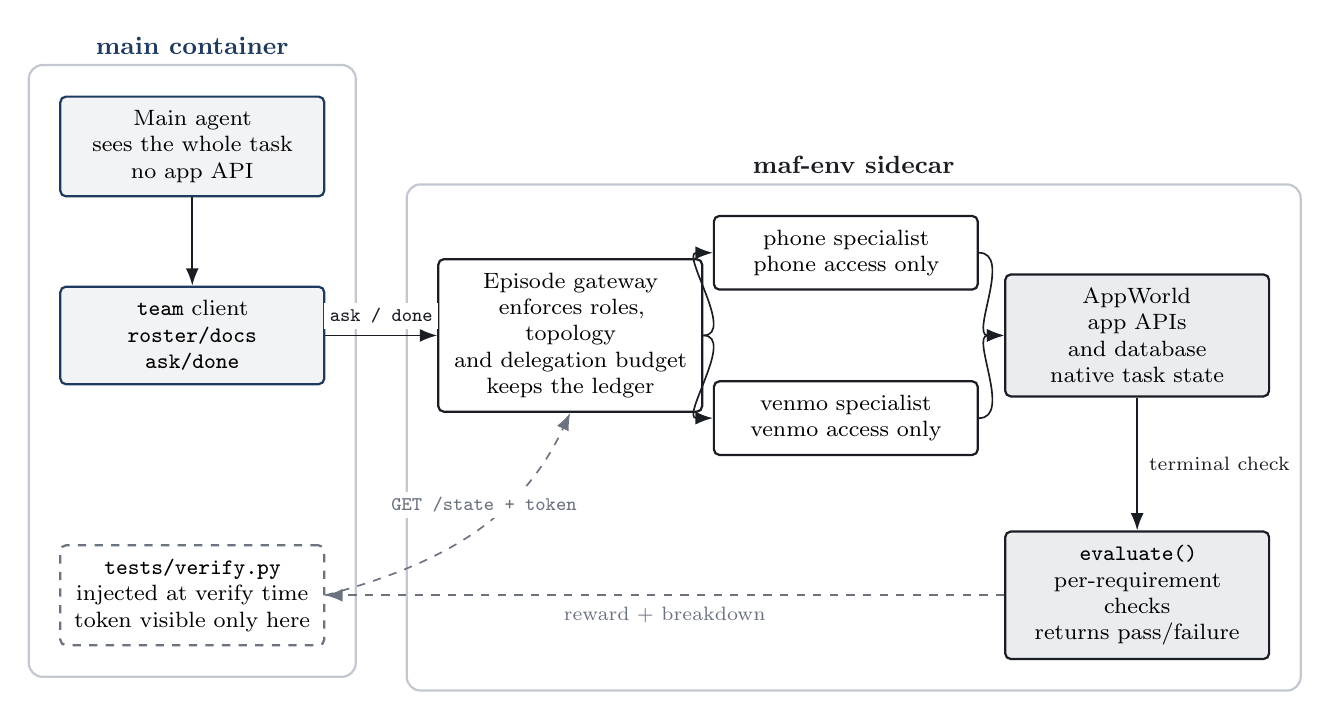
\begin{tikzpicture}[
  font=\footnotesize,
  % Wider than the CJK figure's 2.7cm, and hyphenation off: English box labels
  % broke as "delega-tion budget" and "token visi-ble only here".
  component/.style={draw=rulegray,rounded corners=2pt,fill=white,
    minimum height=0.9cm,text width=3.0cm,align=center,inner sep=5pt,
    execute at begin node={\hyphenpenalty=10000\exhyphenpenalty=10000}},
  main/.style={component,draw=accent,thick,fill=accent!6},
  side/.style={component,draw=ink,thick,fill=white},
  world/.style={component,draw=ink,thick,fill=rulegray!35},
  verify/.style={component,draw=muted,thick,dashed,fill=white},
  boundary/.style={draw=rulegray,rounded corners=5pt,thick,inner sep=11pt},
  edge/.style={-{Latex[length=2.2mm]},semithick,draw=ink},
  verifyedge/.style={-{Latex[length=2.2mm]},semithick,dashed,draw=muted},
  flowlabel/.style={font=\scriptsize,fill=white,inner sep=2pt,text=ink},
  verifylabel/.style={flowlabel,text=muted}
]
  \node[main] (agent) at (0,2.4) {Main agent\\sees the whole task\\no app API};
  \node[main] (team) at (0,0) {\texttt{team} client\\\texttt{roster/docs}\\\texttt{ask/done}};
  \node[verify] (verifier) at (0,-3.3) {\texttt{tests/verify.py}\\injected at verify time\\token visible only here};

  \node[side] (gateway) at (4.8,0) {Episode gateway\\enforces roles, topology\\and delegation budget\\keeps the ledger};
  \node[side] (phone) at (8.3,1.05) {phone specialist\\phone access only};
  \node[side] (venmo) at (8.3,-1.05) {venmo specialist\\venmo access only};
  \node[world] (appworld) at (12.0,0) {AppWorld\\app APIs and database\\native task state};
  \node[world] (judge) at (12.0,-3.3) {\texttt{evaluate()}\\per-requirement checks\\returns pass/failure};

  \node[boundary,fit=(agent)(team)(verifier),
    label={[font=\small\bfseries,text=accent]above:main container}] (mainbox) {};
  \node[boundary,fit=(gateway)(phone)(venmo)(appworld)(judge),
    label={[font=\small\bfseries,text=ink]above:maf-env sidecar}] (sidebox) {};

  \draw[edge] (agent) -- (team);
  \draw[edge] (team.east) -- node[flowlabel,above=2pt]{\texttt{ask / done}} (gateway.west);
  \draw[edge] (gateway.east) to[out=0,in=180] (phone.west);
  \draw[edge] (gateway.east) to[out=0,in=180] (venmo.west);
  \draw[edge] (phone.east) to[out=0,in=180] (appworld.west);
  \draw[edge] (venmo.east) to[out=0,in=180] (appworld.west);
  \draw[edge] (appworld.south) -- node[flowlabel,right=2pt]{terminal check} (judge.north);

  \draw[verifyedge] (verifier.east) to[out=15,in=-115]
    node[verifylabel,pos=0.55,above=2pt]{\texttt{GET /state + token}} (gateway.south);
  \draw[verifyedge] (judge.west) --
    node[verifylabel,below=2pt]{reward + breakdown} (verifier.east);
\end{tikzpicture}
\caption{Container architecture of a Harbor task. The solid box on the left is the main container the model can see; AppWorld, the sub-agents, the ledger and the judging logic all stay in the sidecar. Dashed lines mark the verification phase, which happens only after the agent has finished.}
\label{fig:architecture}
\end{figure}

Two boundaries in Figure~\ref{fig:architecture} matter most. First, the Main's filesystem holds no AppWorld, no ground truth and no verifier; it can only issue natural-language delegations through \texttt{team}. Second, the verifier token never exists during the agent phase; Harbor injects the tests into the main container only after execution ends, and the verifier reads the terminal state from the sidecar. Role constraints are thus enforced by the environment, and the model cannot read its own reward mid-run.

\subsection{How a task runs}

Figure~\ref{fig:trajectory} shows the reference trajectory for task \texttt{2a163ab\_1}. Each \texttt{team ask} in the figure may contain several rounds of sub-agent reasoning and API calls internally; only cross-role information flow is kept here. What decides success is not the number of messages but whether the Main obtains the roommate list first, then hands venmo the names, the date range and the full-pagination requirement together.

\begin{figure}[H]
\centering
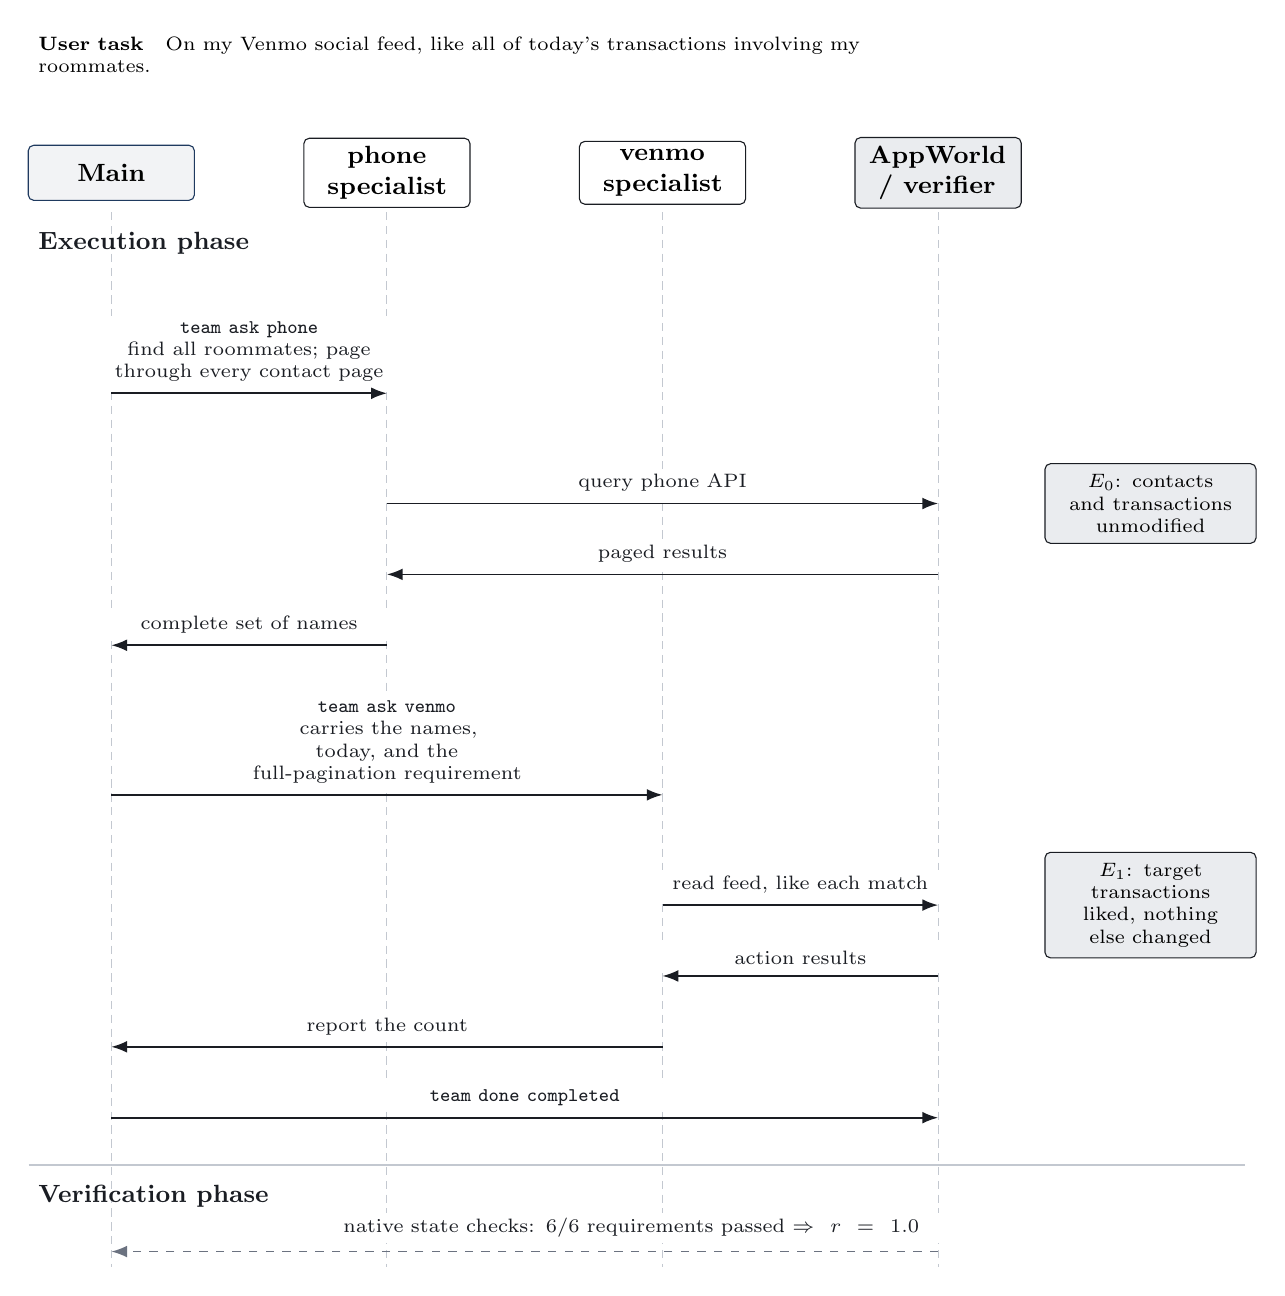
\begin{tikzpicture}[
  font=\footnotesize,
  actor/.style={draw=ink,rounded corners=2pt,minimum width=2.1cm,
    minimum height=0.7cm,align=center,font=\small\bfseries,fill=white,
    text width=1.9cm,inner sep=3pt},
  lifeline/.style={draw=rulegray,densely dashed},
  msg/.style={-{Latex[length=2mm]},semithick,draw=ink},
  % Hyphenation off: these labels are narrow enough that TeX broke "every" as
  % "ev-ery" inside a diagram, where a hyphen reads as part of the label.
  msglabel/.style={font=\scriptsize,fill=white,inner sep=2pt,align=center,
    text=ink,text width=3.7cm,
    execute at begin node={\hyphenpenalty=10000\exhyphenpenalty=10000}},
  state/.style={draw=ink,rounded corners=2pt,fill=rulegray!35,
    text width=2.4cm,align=center,font=\scriptsize,inner sep=4pt},
  phase/.style={font=\small\bfseries,text=ink}
]
  \node[align=left,anchor=west,font=\scriptsize,text width=11cm] (task) at (-1.05,1.5)
    {\textbf{User task}\quad On my Venmo social feed, like all of today's transactions involving my roommates.};

  \node[actor,draw=accent,fill=accent!6] (main) at (0,0) {Main};
  \node[actor] (phone) at (3.5,0) {phone\\specialist};
  \node[actor] (venmo) at (7.0,0) {venmo\\specialist};
  \node[actor,fill=rulegray!35] (world) at (10.5,0) {AppWorld\\/ verifier};

  \foreach \x in {0,3.5,7.0,10.5}
    \draw[lifeline] (\x,-0.5) -- (\x,-13.9);

  \node[phase,anchor=west] at (-1.05,-0.9) {Execution phase};

  \draw[msg] (0,-2.8) -- node[msglabel,above=2pt]
    {\texttt{team ask phone}\\find all roommates; page through every contact page} (3.5,-2.8);

  \draw[msg] (3.5,-4.2) -- node[msglabel,above=2pt]
    {query phone API} (10.5,-4.2);
  \node[state,anchor=west] at (11.85,-4.2)
    {$E_0$: contacts and transactions unmodified};
  \draw[msg] (10.5,-5.1) -- node[msglabel,above=2pt]
    {paged results} (3.5,-5.1);
  \draw[msg] (3.5,-6.0) -- node[msglabel,above=2pt]
    {complete set of names} (0,-6.0);

  \draw[msg] (0,-7.9) -- node[msglabel,above=2pt]
    {\texttt{team ask venmo}\\carries the names, today, and the full-pagination requirement} (7.0,-7.9);

  \draw[msg] (7.0,-9.3) -- node[msglabel,above=2pt]
    {read feed, like each match} (10.5,-9.3);
  \node[state,anchor=west] at (11.85,-9.3)
    {$E_1$: target transactions liked, nothing else changed};
  \draw[msg] (10.5,-10.2) -- node[msglabel,above=2pt]
    {action results} (7.0,-10.2);
  \draw[msg] (7.0,-11.1) -- node[msglabel,above=2pt]
    {report the count} (0,-11.1);
  \draw[msg] (0,-12.0) -- node[msglabel,above=2pt]
    {\texttt{team done completed}} (10.5,-12.0);

  \draw[rulegray,semithick] (-1.05,-12.6) -- (14.4,-12.6);
  \node[phase,anchor=west] at (-1.05,-13.0) {Verification phase};
  \draw[msg,dashed,draw=muted] (10.5,-13.7) -- (0,-13.7);
  % Wide enough for one line, and pushed right of the phase label: at 7cm this
  % wrapped to two lines, and the white fill of its second line sat on top of
  % "Verification phase", clipping it to "Verification ph" in the PDF.
  \node[msglabel,text width=9cm,anchor=south] at (6.6,-13.6)
    {native state checks: 6/6 requirements passed $\Rightarrow r=1.0$};
\end{tikzpicture}
\caption{Information flow of the reference trajectory. Upstream roles only obtain facts; the Main's job is to organise those facts into a complete, executable request for the downstream role. The final reward comes from state $E_1$, not from matching the trajectory text. Dashed lines are the verification phase, after the agent has finished.}
\label{fig:trajectory}
\end{figure}

\subsection{Reward and validity references}

The verifier does not assess whether the conversation was ``sensible'', and it does not take the model's own account of its work. If the task has $N$ state requirements of which $N_{\mathrm{pass}}$ pass, the reward is
\[
  r=\frac{N_{\mathrm{pass}}}{N}.
\]
This keeps partial credit while avoiding an LLM judge. The model may decompose and communicate however it likes; as long as the final state is correct with no extra side effects, it earns the same reward.

To confirm the reward means anything, each configuration needs three references. The first is the reference solution, proving the task is solvable. The second is the unconstrained control, giving a single agent every app, confirming the base task can be completed at all. The third is the do-nothing baseline, measuring how many checks already pass when no action is taken. Only when the constrained group sits between the solvable ceiling and the no-action floor, and produces a non-degenerate distribution across instances, is the task set suitable for RL.

\section{Difficulty Control and Scaling}

\subsection{Which directions difficulty moves along}

Difficulty varies along four directions. First, information visibility: the Main may read each role's capability documentation, or see only role names. Second, dependency structure: a task can grow from a two-step sequential dependency to three apps and multi-branch dependencies. Third, communication constraints, including the delegation budget and the star, chain and tree topologies. Fourth, the operational scale of the task itself --- pages to traverse, entities involved, state modifications required.

These have to be added one layer at a time. A valid difficulty knob must satisfy two conditions: the reference solution still passes reliably, and the model's reward or failure structure changes reproducibly against the previous layer. A topology that merely makes the task unexecutable produces an environment fault, not higher difficulty --- which is how chain got kept out of the delivery (\S\ref{sec:operators}).

\subsection{Batch generation: the free half}

The forging pipeline is four commands, and three of them call no model. \texttt{measure} reads the 147 ground-truth-bearing tasks and parses out which apps each one actually touched. \texttt{seams} runs a forward taint pass over the same reference solutions and keeps the 39 where facts genuinely cross apps. \texttt{render} turns the selected tasks and constraint configurations into Harbor task directories. All three are static analysis plus file writes, and finish on a laptop in minutes.

The reason they are free is written in the equation of \S\ref{sec:wrap}: $W$ acts only on the environment, and $x$ and $J$ are unchanged word for word. Multiplying along the configuration dimension therefore creates no new design work --- one more visibility setting is one more pass of writing task directories. With 39 tasks and 2 implemented configurations, a single \texttt{render} command writes 78 task directories, plus an unconstrained control per task.

The real question is how many of those 78 directories can ship. The next two sections are the two costs, both downstream of \texttt{render}.

\subsection{Cost one: reference solutions are currently hand-written}
\label{sec:refcost}

A Harbor task ships a \texttt{solution/} to prove it is solvable, and the reference solution here is not a script replay. The specialists are real LLMs, and the Main's job is to decompose rather than to execute, so a reference path records only the decomposition itself: ask phone for the names, then hand the names to venmo, with the specialists still doing the actual work. That makes this oracle probabilistic: verification needs live model calls and can fail on a bad specialist turn. That is a cost, stated rather than hidden. These paths are currently written one at a time, and \texttt{REFERENCE\_PATHS} holds only 3 --- a single task family. Running \texttt{render} over 39 tasks today writes 78 directories, of which \textbf{72 ship a \texttt{solve.sh} that fails loudly and says why}: a task with no reference solution cannot be proved solvable and therefore cannot enter a training set. This is the step standing furthest between here and ``large batches''.

But it can be automated, and the skeleton has already been computed. To measure selection yield at all, \texttt{seams.py} already has to answer ``which app produced the fact, and which app's action consumed it''. A reference path records that same triple: render (producer, fact, consumer) into (ask the producer, hand the fact to the consumer), and that is the whole structure of the path.

What remains by hand is not per-task authorship but per-app calling technique. Every brief, for instance, has to say ``page through to the end'' --- that is phone's and venmo's pagination semantics, not a property of any one task. Such techniques count per app, not per task: 6 apps' worth in total, amortised across every task, which is a constant. This is measured, not hoped for --- chasing down the ``random'' flake on \texttt{2a163ab\_3} showed phone stopping at page one and dropping a coworker, not bad luck, and one added sentence about pagination fixed it for good (\texttt{reference.py} records the investigation). The shape of this cost is therefore: write the calling conventions for 6 apps once, then render per seam --- not write 39 of them.

\subsection{Cost two: verification, and it grows linearly in configurations}

Verification cannot be free, because validity is a property of the rollout distribution rather than of a single draw (\S\ref{sec:yield}). A cell's yield needs \texttt{SEEDS\_FOR\_YIELD} $=5$ replicates before it counts as measured, and the arithmetic follows directly: 39 tasks $\times$ 2 configurations $\times$ 5 seeds $=390$ constrained rollouts, plus $39\times5=195$ controls, for 585 in total. At the per-run times the existing sweep measured (173 s mean across the two star settings, 30 s for the control), that is roughly 20 hours serial, or about 1.3 hours at 16-way parallelism.

So compute is not the wall. Two other things are. First, the real ceiling is usually API rate rather than compute: the same cells stretched from about 200 s to 6{,}700--15{,}000 s under rate limiting, a factor of 30--75 (\code{sweep/appworld_rate_limit_cost.json}). Second, this term grows linearly in the number of configurations --- every new knob has to be re-run across every task with a full set of seeds before anyone knows whether that knob is difficulty or a fault. This is exactly the argument for measuring yield before scaling out: expanding on a configuration that has not been shown to produce a training signal expands invalid data.

\subsection{The ceiling: this dimension holds only 13 independent task families}
\label{sec:ceiling}

Even with both costs solved, the source itself has a hard ceiling, and it is far below 39.

The 39 seam-bearing tasks are not 39 independent samples: they are \textbf{13 task families of 3 variants each}. Variants share a dependency structure and differ only in entity, date and operational scale --- the shipped \texttt{2a163ab\_1/2/3} are three variants of one family, asking about roommates, siblings and coworkers respectively. By app combination the concentration is worse still (Table~\ref{tab:combos}): 24 tasks across 8 families are phone+venmo.

\begin{table}[H]
\centering
\small
\caption{App-combination distribution of the 39 seam-bearing tasks (\texttt{sweep/appworld\_seams.json})}
\label{tab:combos}
\begin{tabularx}{\textwidth}{X c c}
\toprule
App combination & Tasks & Families\\
\midrule
phone + venmo & 24 & 8\\
phone + simple\_note + venmo & 3 & 1\\
simple\_note + spotify & 3 & 1\\
file\_system + phone + venmo & 3 & 1\\
phone + splitwise + venmo & 3 & 1\\
file\_system + simple\_note & 3 & 1\\
\midrule
Total & \textbf{39} & \textbf{13}\\
\bottomrule
\end{tabularx}
\end{table}

One more layer tightens it further: AppWorld has 9 apps, but the 147 ground-truth-bearing tasks touch only 6 of them, and the seam-bearing tasks use only 6 combinations. So the trainable diversity on this dimension is 13 families and 6 combinations --- not 39 tasks, and certainly not 78 directories. The abstract's ``configuration count is not task count'' needs one more turn of the screw here: \textbf{task count is not family count either}. To make the data volume actually grow, what is missing is not a knob. It is source tasks.

\subsection{The admission test: what the method asks of a database}
\label{sec:substrate}

AppWorld is an argument to this method, not a premise of it. The method asks four things of a database, and dropping any one collapses it back into ``design your own verifier'' --- which \S\ref{sec:invariant} argues is forbidden by the very reason the method exists:

\begin{enumerate}[leftmargin=*,itemsep=0.15em]
\item \textbf{A programmatic verifier you did not write.} It is what makes the reward batch-computable, and what excuses you from ever defending a judgement about ``how well they collaborated''. Its value is precisely that somebody else already validated it.
\item \textbf{Real, executable, installable.} Not a description of a world. A database you cannot \texttt{pip install} or \texttt{docker pull} is one you will finish by building --- and then you designed it, and requirement 1 is gone with it.
\item \textbf{A reference solution per task.} It serves two purposes: deriving the roster (the roles come from the tools the reference solution touched, not from the designer's hand) and proving solvability. Only 147 of AppWorld's 750 tasks carry ground truth, and that is where the number 147 comes from.
\item \textbf{A tool boundary that can be cut.} The permission partition is the most fundamental of the four constraints (\S\ref{sec:wrap}): if the tools cannot be split by role, the Main can bypass coordination and finish alone, and the other three become moot.
\end{enumerate}

\textbf{Admission is necessary and not sufficient.} A database can clear all four and still yield nothing, because none of the four measures how \emph{deep} the seams run: it may ship a flawless verifier and have every task collapse onto a single role. That is why seam analysis (\S\ref{sec:select}) is a measurement rather than an assumption, and AppWorld nearly makes the point by itself --- 96 of its 147 ground-truth tasks are single-app puzzles. The seams are also where substrate choice stops being free: SWE-smith has the strongest verifier on the list and scaled on the strength of requirement 1~\cite{yang2025swesmith}, but its seams are code modules, so partitioning it yields a software-engineering task with extra agents rather than an orchestration task.

\textbf{How far this generalises, stated honestly.} Nothing in the method is AppWorld-shaped: the admission test is a property of a database, the roster is read off whatever a reference solution touches, the constraints act on an access surface, and the validity rule (\S\ref{sec:criterion}) needs only a score, a floor and a control. But that is an argument from construction --- checkable by reading it --- and not a result. \textbf{This method has been run end to end on exactly one database.} The reach claimed here is therefore the admission test's: any database clearing all four requirements should work, and one has. A second substrate is the cheapest available falsification, and it has not been run; \S\ref{sec:next} treats that as a task rather than a caveat. The order for scaling up is: automate reference solutions out of the seams, measure yield on the 13 families that exist, and then widen sideways to new source databases --- rather than piling more configurations onto the same task family.

\section{Data Samples and Experimental Results}
\label{sec:results}

The minimal delivery sample is three instances from one task family. All three require obtaining a class of contacts from phone first, then having venmo act on the related transactions within a date range. They test the same capability structure but differ in entity, date and operational scale.

\begin{table}[H]
\centering
\small
\caption{Three Harbor data samples}
\begin{tabularx}{\textwidth}{>{\raggedright\arraybackslash}p{2.1cm} X >{\raggedright\arraybackslash}p{4.6cm}}
\toprule
Task ID & User task & Required coordination\\
\midrule
\texttt{2a163ab\_1} & Like all of today's transactions involving roommates on the Venmo social feed & phone finds the roommates' names; venmo pages today's feed and likes\\
\texttt{2a163ab\_2} & Like all of yesterday's transactions involving siblings on the Venmo social feed & phone finds the siblings' names; venmo pages yesterday's feed and likes\\
\texttt{2a163ab\_3} & Like all transactions involving coworkers from yesterday or today on the Venmo social feed & phone finds the coworkers' names; venmo pages across two dates and likes\\
\bottomrule
\end{tabularx}
\end{table}

All three samples' Harbor reference solutions pass all 6 state checks for a reward of 1.0. We then compare three configurations on the same tasks: open as the unconstrained control; star-docs, which forces the Main to delegate but lets it read the roles' capabilities; and star-names, which further hides the capability docs and leaves only role names. The Main uses \texttt{gpt-5.6-sol} and the specialists \texttt{gpt-4.1}, with one seed per cell so far.

\begin{table}[H]
\centering
\small
\caption{Constraint ablation results}
\label{tab:results}
\begin{tabularx}{\textwidth}{>{\raggedright\arraybackslash}p{2.65cm} c c c X}
\toprule
Configuration & Mean reward & Three tasks & Mean time/s & Meaning\\
\midrule
open & 1.000 & 1.000/1.000/1.000 & 30.2 & one agent holds every app\\
star-docs & 0.944 & 1.000/1.000/0.833 & 200.8 & delegation forced; the roles' real API catalogue is readable\\
star-names & 0.445 & 1.000/0.167/0.167 & 145.9 & delegation forced; role capabilities invisible\\
\midrule
do-nothing & 0.333 & 0.333/0.333/0.333 & --- & no action taken, but the answer type is right\\
\bottomrule
\end{tabularx}
\end{table}

Neither knob in this table is what its name says, so each needs taking apart.

star-docs drops only 0.056 against open --- a strong model can reach the goal through a few delegations even without direct tools. More notable: the Main in this setting previously received the sentence ``their capabilities are listed above'' while \emph{nothing} was above it but two role names. The thing that actually served the catalogue was \texttt{team docs} in the delivered container, while the measurement went down a different in-process path (see \S\ref{sec:boundary}). After this round put the real API catalogues --- 2{,}838 and 5{,}444 characters --- in front of the Main, the score did not move at all: still 0.944. What moved was the delegation count, from 2--3 up to 3--5, and the time, from 100 s to 201 s. In other words, letting the Main see what the sub-agents can do bought more delegations and more latency, but no more success.

star-names' $0.944\rightarrow0.445$ looks at last like visibility biting. It is not. Two of its three cells score $0.167$ --- below the 0.333 ``floor''. They got there like this: the Main failed to find the target transactions and \emph{honestly reported} that there were none matching, while AppWorld's \texttt{assert answers match} expects an action task's answer (\texttt{None}); prose does not match, so that requirement fails. Had the Main lied and claimed \texttt{completed}, it would have scored 0.333.

This does not have to be inferred from the sweep. It can be measured directly, with no model calls at all: open the same task, do nothing, vary only the submitted answer, and evaluate. \code{appworld_protocol_probe.py} does exactly that, with results in \code{sweep/appworld_protocol.json}.

\begin{table}[H]
\centering
\small
\caption{Same non-work, different words. Consistent across all three tasks, no model calls.}
\label{tab:protocol}
\begin{tabularx}{\textwidth}{X c X}
\toprule
Agent & Score & Requirements lost\\
\midrule
do nothing, claim \texttt{completed} falsely & \textbf{0.333} & 4 state checks\\
do nothing, honestly report ``found none'' & \textbf{0.167} & the same 4, \emph{plus} \texttt{assert answers match}\\
\bottomrule
\end{tabularx}
\end{table}

Both agents did exactly the same work (none), the terminal world state is identical, and the same four state checks fail. The only difference is \emph{how they describe themselves}, and that difference is worth $1/6$.

\begin{quote}
\small
\noindent \textbf{This reward pays $1/6$ for a false claim of completion.} For a policy in training, that means lying about completion is strictly better than reporting failure honestly.
\end{quote}

It also means the label ``do-nothing $=0.333$'' in Table~\ref{tab:results} is wrong: that is not a floor but the score for ``got the answer type right while doing nothing'', and an honest failure can land beneath it.

To be clear, \textbf{this method cannot fix it}. The verifier is AppWorld's, and changing it means starting to design verifiers --- the one thing forbidden by the entire argument of \S\ref{sec:invariant} for why this method exists. What can be done is to measure it, report it, and --- before training on this data --- split the reward into a state term and a protocol term, recording them separately and driving the policy with the former only. The current $r=N_{\mathrm{pass}}/N$ mixes the two into one scalar, and every difficulty curve in this report before this point is contaminated by it.

The current data is therefore \textbf{insufficient} to support the claim that hiding role capabilities is the more effective source of difficulty. Under the sandwich criterion of \S\ref{sec:yield}, star-names yields 0/3 usable cells, still below star-docs' 1/3.

\section{Discussion and Extensions}

\subsection{Shore up the existing conclusions first}
\label{sec:verifyfirst}
\label{sec:next}

The current results remain a small-scale validation. The three instances come from one task family and each configuration has a single seed, so 0.056 and 0.167 cannot yet be treated as stable effects. The first next step is to add seeds on the existing tasks and give interval estimates for the differences; after that, add phone--simple\_note, file\_system--spotify and three-app tasks to confirm the conclusions hold across task types.

There is a second gap of a different kind, and it is cheaper to close than any of the above: \textbf{the method is presented as substrate-independent and has been run on one substrate} (\S\ref{sec:substrate}). Seam analysis is the part that transfers most obviously and costs the least to check --- it needs no rollouts and no model calls, only reference solutions --- so running it against a second admitted database and publishing the seam distribution would either corroborate the generality claim or refute it for the price of an afternoon. Until somebody does, the claim rests on reading the construction rather than on evidence, and this report marks it as such rather than letting the survey of candidate databases do work that only a measurement can do.

Beyond that, the current reward reliably judges whether the final task was completed but cannot separate failures of decomposition, role selection and communication. That is also why this stage does not list Theory of Mind and dynamic recovery as separate dimensions. Finer-grained capability attribution can be done through paired probes or environment-side fault injection, but it should still be verified from the final state rather than falling back on scoring the conversation.

Once star-names' effect is stable across multiple seeds and task families, adding delegation budgets and chain/tree topologies becomes reasonable. That way each curriculum level builds on capabilities already mastered at the level below, and difficulty changes are easier to explain.

\subsection{From spatial constraints to temporal ones}

The current work changes the spatial structure of collaboration: who holds which tools, who knows what, along which topology messages may travel. The next stage can add a time axis to the same environment, so that information is not handed over all at once at the start but appears when the agent asks for it or when the task reaches a particular state. That would train hidden-requirement discovery and dynamic replanning under user intervention, without giving up terminal-state verification.

A minimal version generates paired samples from the same complete task. The control group still receives the full instruction; the experimental group receives a deliberately incomplete but realistically phrased request, with the contact scope, date or compatibility preference held in hidden user state in the sidecar. The Main can obtain those constraints only by noticing the gap and asking the user. Both groups share an initial world and a final verifier, so there is no need to score ``was that a good question?'' separately: if the key question never gets asked, the agent cannot reliably reach the correct terminal state; and asking about everything burns a limited interaction budget.

User intervention can serve as the next difficulty layer. After the agent has done part of the work, simulate the user adding a changed scope or a new restriction, requiring the Main to update the plan, keep the results that remain valid, and pass the new constraint to the relevant roles. Two cases must be distinguished here: if the added information was always part of the original goal and merely unstated, the final judge can stay unchanged; if the user genuinely changed the goal, the new terminal state needs an equally trustworthy environment check, and cannot be judged from the conversation alone.

This temporal extension can be written as
\[
  \tau_{c,h}=(x_0,\mathcal{E}_c,U_h,\Gamma_h,J),
\]
where $U_h$ is hidden user state existing only in the sidecar and $\Gamma_h$ decides when information is asked for, revealed or modified. The project's most important boundary still has to hold: hidden state must never enter the Main's filesystem, the interaction record must not be forgeable by the agent, and the final reward must continue to come from replayable environment state. Only once paired experiments reliably separate the scores of full instruction, hidden requirement and mid-run intervention should it enter a formal curriculum.

\section{Conclusion}

The key to this method is not inventing new tasks out of nothing. It is finding coordination dependencies inside real tasks that already exist, then making those dependencies explicit through permission and information allocation. The Main must plan and delegate, the sub-agents can only do local work, and the final reward still comes from AppWorld's real world state.

Configurations can therefore be generated in bulk and the verification logic reused. But \textbf{whether difficulty can be tuned along these directions is not something this report has proved}. What the three samples prove is that the partitioned environment and the Harbor verifier run correctly, and that reference solutions pass all 6 state checks. Beyond that, the existing sweep observed a non-degenerate training signal in exactly one star-docs instance; star-names is not an established difficulty increment (\S\ref{sec:results}), the chain topology is not built, and parallel scheduling is out of scope.

What comes next is therefore not scaling up but making this one cell solid: add seeds to the shipped configurations, strip the submission protocol's contamination out of the reward, and extend the delivered samples from one task family to different dependency structures. Hidden user requirements and mid-run intervention are worthwhile extensions, but they should sit on top of a base configuration already proven to produce a training signal reliably --- and no such configuration exists yet.

\begingroup
\footnotesize
\begin{thebibliography}{9}
\setlength{\itemsep}{0.25em}
\setlength{\parskip}{0pt}

\bibitem{trivedi2024appworld}
Harsh Trivedi et al.
\newblock AppWorld: A Controllable World of Apps and People for Benchmarking Interactive Coding Agents.
\newblock \emph{ACL 2024}, arXiv:2407.18901.
\newblock \url{https://arxiv.org/abs/2407.18901}

\bibitem{yang2025swesmith}
John Yang, Kilian Lieret, Carlos E. Jimenez, et al.
\newblock SWE-smith: Scaling Data for Software Engineering Agents.
\newblock arXiv:2504.21798, 2025.
\newblock \url{https://arxiv.org/abs/2504.21798}

\bibitem{zhu2025multiagentbench}
Kunlun Zhu, Hongyi Du, Zhaochen Hong, et al.
\newblock MultiAgentBench: Evaluating the Collaboration and Competition of LLM Agents.
\newblock \emph{ACL 2025}, arXiv:2503.01935.
\newblock \url{https://arxiv.org/abs/2503.01935}

\bibitem{cemri2025mast}
Mert Cemri, Melissa Z. Pan, Shuyi Yang, et al.
\newblock Why Do Multi-Agent LLM Systems Fail?
\newblock arXiv:2503.13657, 2025.
\newblock \url{https://arxiv.org/abs/2503.13657}

\bibitem{harbor2026tasks}
Harbor Framework.
\newblock Task Structure: Creating and Running Tasks for Agentic Environments.
\newblock Documentation, accessed 2026-07-16.
\newblock \url{https://www.harborframework.com/docs/tasks}

\end{thebibliography}
\endgroup

\end{document}
